
\begin{figure}[h]

\centering




\tikzset{every picture/.style={line width=0.75pt}} %set default line width to 0.75pt        

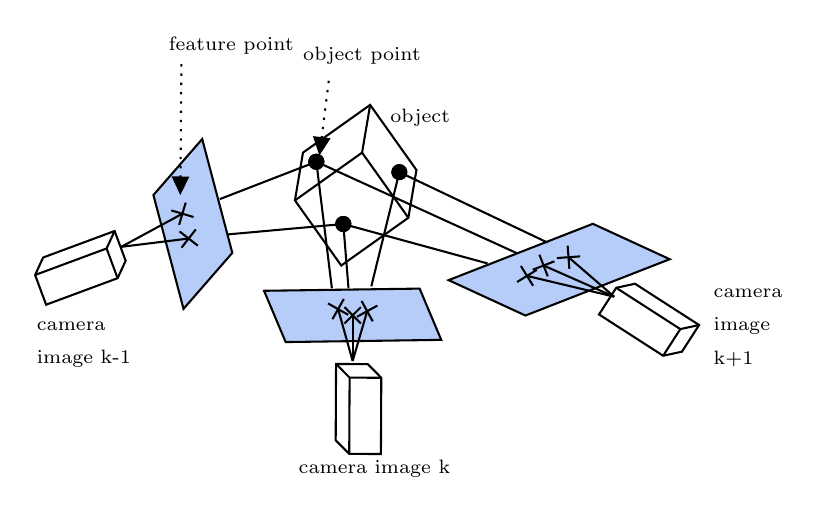
\begin{tikzpicture}[x=0.75pt,y=0.75pt,yscale=-1,xscale=1]
%uncomment if require: \path (0,300); %set diagram left start at 0, and has height of 300

\draw   (142.51,155.56) -- (146.37,147.14) -- (180.82,134.37) -- (186.13,148.7) -- (182.26,157.11) -- (147.82,169.88) -- cycle ; \draw   (180.82,134.37) -- (176.95,142.79) -- (142.51,155.56) ; \draw   (176.95,142.79) -- (182.26,157.11) ;
\draw   (293.85,241.75) -- (287.33,235.17) -- (287.51,198.43) -- (302.79,198.51) -- (309.3,205.09) -- (309.12,241.82) -- cycle ; \draw   (287.51,198.43) -- (294.03,205.01) -- (293.85,241.75) ; \draw   (294.03,205.01) -- (309.3,205.09) ;
\draw   (422.48,161.74) -- (431.53,159.78) -- (462.42,179.67) -- (454.15,192.51) -- (445.1,194.47) -- (414.21,174.58) -- cycle ; \draw   (462.42,179.67) -- (453.37,181.63) -- (422.48,161.74) ; \draw   (453.37,181.63) -- (445.1,194.47) ;
\draw   (267.69,119.63) -- (271.57,96.62) -- (303.93,73.61) -- (326.24,104.98) -- (322.35,127.99) -- (290,151) -- cycle ; \draw   (303.93,73.61) -- (300.04,96.62) -- (267.69,119.63) ; \draw   (300.04,96.62) -- (322.35,127.99) ;
\draw    (231.5,119) -- (278,101) ;
\draw [shift={(278,101)}, rotate = 338.84] [color={rgb, 255:red, 0; green, 0; blue, 0 }  ][fill={rgb, 255:red, 0; green, 0; blue, 0 }  ][line width=0.75]      (0, 0) circle [x radius= 3.35, y radius= 3.35]   ;

\draw    (235.5,136) -- (291,131) ;
\draw [shift={(291,131)}, rotate = 354.85] [color={rgb, 255:red, 0; green, 0; blue, 0 }  ][fill={rgb, 255:red, 0; green, 0; blue, 0 }  ][line width=0.75]      (0, 0) circle [x radius= 3.35, y radius= 3.35]   ;

\draw    (285.5,162) -- (278,101) ;
\draw [shift={(278,101)}, rotate = 262.99] [color={rgb, 255:red, 0; green, 0; blue, 0 }  ][fill={rgb, 255:red, 0; green, 0; blue, 0 }  ][line width=0.75]      (0, 0) circle [x radius= 3.35, y radius= 3.35]   ;

\draw    (293.5,162) -- (291,131) ;
\draw [shift={(291,131)}, rotate = 265.39] [color={rgb, 255:red, 0; green, 0; blue, 0 }  ][fill={rgb, 255:red, 0; green, 0; blue, 0 }  ][line width=0.75]      (0, 0) circle [x radius= 3.35, y radius= 3.35]   ;

\draw    (304.5,161) -- (318,106) ;
\draw [shift={(318,106)}, rotate = 283.79] [color={rgb, 255:red, 0; green, 0; blue, 0 }  ][fill={rgb, 255:red, 0; green, 0; blue, 0 }  ][line width=0.75]      (0, 0) circle [x radius= 3.35, y radius= 3.35]   ;

\draw    (360.5,150) -- (291,131) ;
\draw [shift={(291,131)}, rotate = 195.29] [color={rgb, 255:red, 0; green, 0; blue, 0 }  ][fill={rgb, 255:red, 0; green, 0; blue, 0 }  ][line width=0.75]      (0, 0) circle [x radius= 3.35, y radius= 3.35]   ;

\draw    (389.5,140) -- (318,106) ;
\draw [shift={(318,106)}, rotate = 205.43] [color={rgb, 255:red, 0; green, 0; blue, 0 }  ][fill={rgb, 255:red, 0; green, 0; blue, 0 }  ][line width=0.75]      (0, 0) circle [x radius= 3.35, y radius= 3.35]   ;

\draw    (374.5,145) -- (278,101) ;
\draw [shift={(278,101)}, rotate = 204.51] [color={rgb, 255:red, 0; green, 0; blue, 0 }  ][fill={rgb, 255:red, 0; green, 0; blue, 0 }  ][line width=0.75]      (0, 0) circle [x radius= 3.35, y radius= 3.35]   ;

\draw [rotate around= { 311.07: (218.51, 130.98)
    }] [fill={rgb, 255:red, 114; green, 159; blue, 241 }  ,fill opacity=0.52 ] (216.53,107.5) -- (252.31,107.5) -- (220.5,154.46) -- (184.72,154.46) -- cycle ;
\draw    (184,142) -- (213.48,126.04) ;
\draw [shift={(213.48,126.04)}, rotate = 376.57] [color={rgb, 255:red, 0; green, 0; blue, 0 }  ][line width=0.75]    (-5.59,0) -- (5.59,0)(0,5.59) -- (0,-5.59)   ;

\draw    (184,142) -- (216.5,138) ;
\draw [shift={(216.5,138)}, rotate = 397.98] [color={rgb, 255:red, 0; green, 0; blue, 0 }  ][line width=0.75]    (-5.59,0) -- (5.59,0)(0,5.59) -- (0,-5.59)   ;

\draw [rotate around= { 247.14: (295.5, 175)
    }] [fill={rgb, 255:red, 114; green, 159; blue, 241 }  ,fill opacity=0.52 ] (296.17,140.26) -- (322.98,140.26) -- (294.83,209.74) -- (268.02,209.74) -- cycle ;
\draw    (295.5,175) -- (295.5,197) ;

\draw [shift={(295.5,175)}, rotate = 135] [color={rgb, 255:red, 0; green, 0; blue, 0 }  ][line width=0.75]    (-5.59,0) -- (5.59,0)(0,5.59) -- (0,-5.59)   ;
\draw    (302.5,173) -- (295.5,197) ;

\draw [shift={(302.5,173)}, rotate = 151.26] [color={rgb, 255:red, 0; green, 0; blue, 0 }  ][line width=0.75]    (-5.59,0) -- (5.59,0)(0,5.59) -- (0,-5.59)   ;
\draw    (288.5,172) -- (295.5,197) ;

\draw [shift={(288.5,172)}, rotate = 119.36] [color={rgb, 255:red, 0; green, 0; blue, 0 }  ][line width=0.75]    (-5.59,0) -- (5.59,0)(0,5.59) -- (0,-5.59)   ;
\draw [rotate around= { 24.74: (395, 153)
    }] [fill={rgb, 255:red, 114; green, 159; blue, 241 }  ,fill opacity=0.52 ] (400.51,126.13) -- (441.27,126.13) -- (389.49,179.87) -- (348.73,179.87) -- cycle ;
\draw    (421.5,166) -- (399.5,147) ;
\draw [shift={(399.5,147)}, rotate = 265.82] [color={rgb, 255:red, 0; green, 0; blue, 0 }  ][line width=0.75]    (-5.59,0) -- (5.59,0)(0,5.59) -- (0,-5.59)   ;

\draw    (421.5,166) -- (387.5,151) ;
\draw [shift={(387.5,151)}, rotate = 248.81] [color={rgb, 255:red, 0; green, 0; blue, 0 }  ][line width=0.75]    (-5.59,0) -- (5.59,0)(0,5.59) -- (0,-5.59)   ;

\draw    (421.5,166) -- (379.5,156) ;
\draw [shift={(379.5,156)}, rotate = 238.39] [color={rgb, 255:red, 0; green, 0; blue, 0 }  ][line width=0.75]    (-5.59,0) -- (5.59,0)(0,5.59) -- (0,-5.59)   ;

\draw  [dash pattern={on 0.84pt off 2.51pt}]  (213,54) -- (212.5,115.04) ;
\draw [shift={(212.48,117.04)}, rotate = 270.47] [fill={rgb, 255:red, 0; green, 0; blue, 0 }  ][line width=0.75]  [draw opacity=0] (8.93,-4.29) -- (0,0) -- (8.93,4.29) -- cycle    ;

\draw  [dash pattern={on 0.84pt off 2.51pt}]  (284,62) -- (279.73,96.06) ;
\draw [shift={(279.48,98.04)}, rotate = 277.15] [fill={rgb, 255:red, 0; green, 0; blue, 0 }  ][line width=0.75]  [draw opacity=0] (8.93,-4.29) -- (0,0) -- (8.93,4.29) -- cycle    ;


\draw (486,181) node  [align=left] {{\scriptsize camera }\\{\scriptsize image}\\{\scriptsize  k+1}};
\draw (306,249) node  [align=left] {{\scriptsize camera image k}};
\draw (166,189) node  [align=left] {{\scriptsize camera }\\{\scriptsize image k-1}};
\draw (237,45) node  [align=left] {{\scriptsize feature point}};
\draw (300,50) node  [align=left] {{\scriptsize object point}};
\draw (328,80) node  [align=left] {{\scriptsize object}};


\end{tikzpicture}



\caption{SFM  Camera Setup Diagram}
\end{figure}